\documentclass[12pt,a4paper]{article}

\usepackage[utf8]{inputenc}
\usepackage[T1]{fontenc}
\usepackage{geometry}
\usepackage{xcolor}
\usepackage{titlesec}
\usepackage{tcolorbox}
\usepackage{enumitem}
\usepackage{hyperref}
\usepackage{longtable}
\usepackage{array}
\usepackage{booktabs}
\usepackage{tikz}
\usetikzlibrary{arrows.meta,positioning,shapes.geometric,fit,calc}

\geometry{margin=1in}
\setlength{\parskip}{0.45em}
\setlength{\parindent}{0pt}

% Color palette
\definecolor{primary}{HTML}{1F4E79}
\definecolor{secondary}{HTML}{2E86AB}
\definecolor{accent}{HTML}{117A65}
\definecolor{lightbg}{HTML}{F4F8FB}
\definecolor{warn}{HTML}{B03A2E}
\definecolor{softgreen}{HTML}{EAF7F2}
\definecolor{softblue}{HTML}{EBF3FA}

\hypersetup{
    colorlinks=true,
    linkcolor=primary,
    urlcolor=secondary
}

\titleformat{\section}
{\large\bfseries\color{primary}}{\thesection}{0.75em}{}
\titleformat{\subsection}
{\normalsize\bfseries\color{secondary}}{\thesubsection}{0.75em}{}

\newtcolorbox{highlightbox}{
    colback=lightbg,
    colframe=secondary,
    boxrule=0.8pt,
    arc=2mm
}

\begin{document}

\begin{titlepage}
    \centering
    {\scshape\LARGE Detailed Project Report \par}
    \vspace{1cm}
    {\huge\bfseries\color{primary}Firm Management System\par}
    \vspace{0.8cm}
    {\Large\color{secondary}C++ Console Application\par}
    \vspace{1.2cm}

    \begin{tcolorbox}[colback=lightbg,colframe=primary,width=0.9\textwidth,arc=2mm]
        \centering
        \textbf{Project Type:} Academic / Practice Project\\
        \textbf{Language:} C++\\
        \textbf{Platform:} Windows Console\\
        \textbf{Repository Folder:} \texttt{c++\_practice}
    \end{tcolorbox}

    \vfill
    {\large Date: \today\par}
\end{titlepage}

\tableofcontents
\newpage

\section{Introduction}
This project is a console-based \textbf{Firm Management System} developed in C++ to manage common business operations in a structured and user-specific way. The system combines a menu-driven console interface, mouse-interactive buttons, file-based persistence, and object-oriented design.

\textbf{Core user capabilities:}
\begin{itemize}[leftmargin=1.4em]
    \item Account creation and authentication (Sign Up / Log In)
    \item Income entry and review
    \item Expense entry and review
    \item Employee registration, listing, removal, and payment status management
    \item Stock item add/update/remove and stock viewing
\end{itemize}

\section{Problem Statement and Motivation}
Small business operations are often managed manually or scattered across notebooks and simple spreadsheets. This creates issues such as:
\begin{itemize}[leftmargin=1.4em]
    \item Data fragmentation across finance, employee, and stock records
    \item Lack of simple authentication and user-specific data separation
    \item Repetitive manual calculations and record tracking
    \item No unified workflow for day-to-day operations
\end{itemize}

The motivation behind this project is to implement a single lightweight desktop-console solution that centralizes these tasks while practicing practical C++ software engineering.

\section{Project Objectives}
\begin{itemize}[leftmargin=1.4em]
    \item Build a complete menu-driven management program in C++.
    \item Apply OOP concepts: abstraction, inheritance, polymorphism, encapsulation.
    \item Use file handling to preserve records between executions.
    \item Design reusable UI components for console interaction.
    \item Organize code into modular feature-based files.
\end{itemize}

\section{Technology and Environment}
\begin{longtable}{|p{4.5cm}|p{9.5cm}|}
\hline
\rowcolor{lightbg}
\textbf{Component} & \textbf{Details} \\
\hline
Language & C++ \\
\hline
Interface & Windows Console UI \\
\hline
Input Model & Mouse event handling (Windows API console input) \\
\hline
Storage & Text and binary files (\texttt{.txt}, \texttt{.bin}) \\
\hline
Programming Paradigm & Object-Oriented + Modular procedural flow \\
\hline
Utilities & ANSI color formatting utilities \\
\hline
\end{longtable}

\section{System Architecture}
\subsection{High-Level Architecture Diagram}
\begin{center}
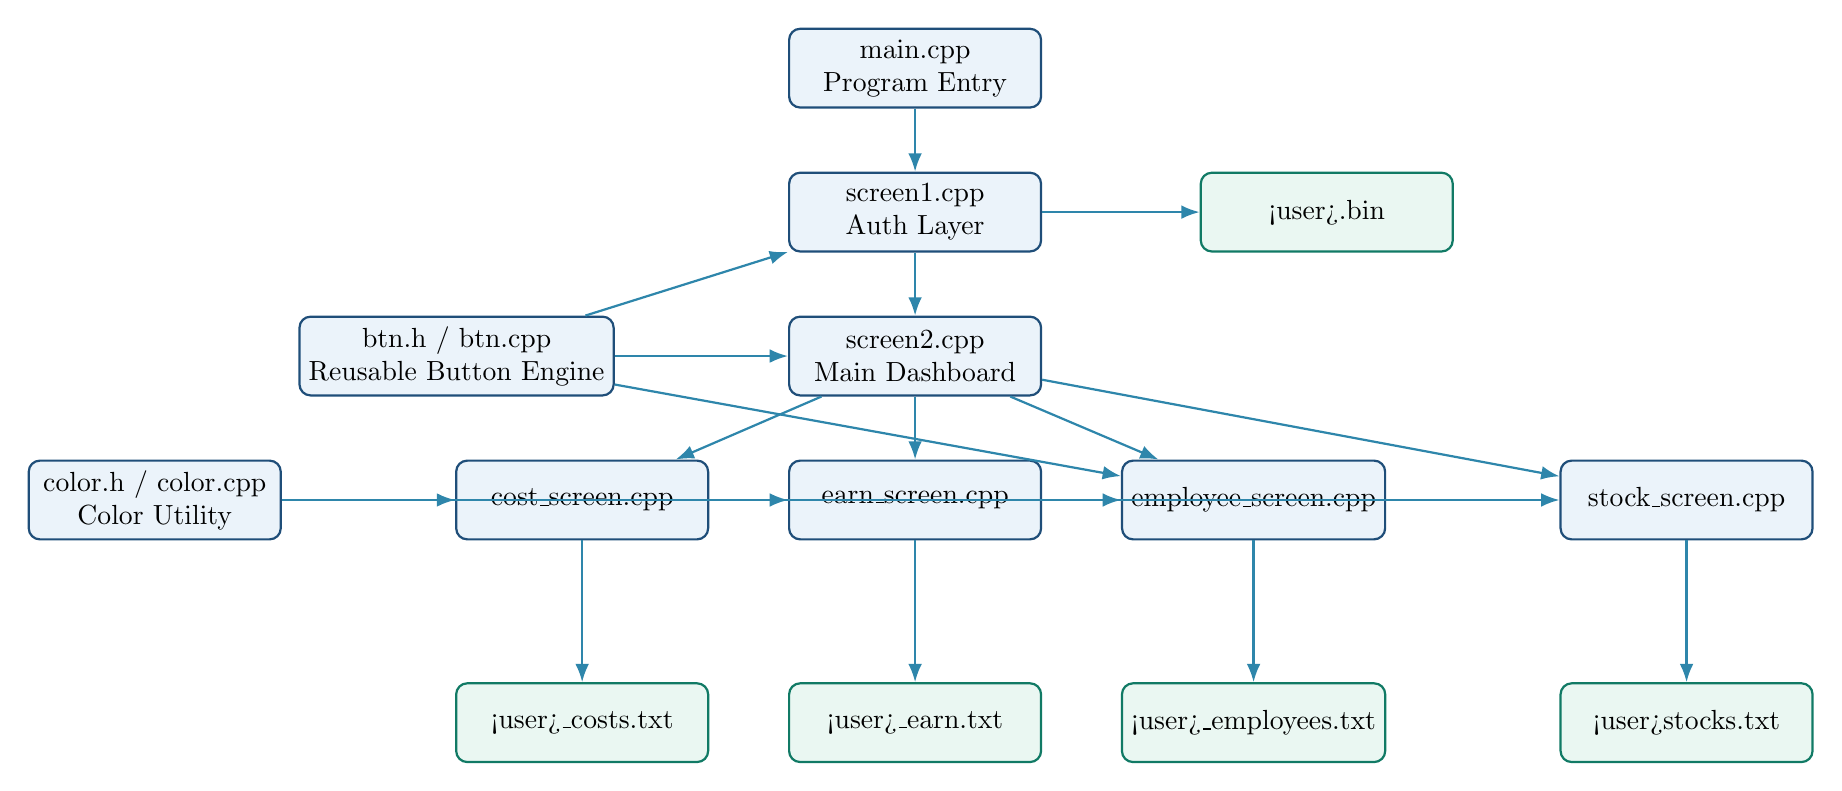
\begin{tikzpicture}[
    node distance=8mm and 10mm,
    box/.style={draw=primary,rounded corners,thick,align=center,minimum height=10mm,minimum width=32mm,fill=softblue},
    datastore/.style={draw=accent,rounded corners,thick,align=center,minimum height=10mm,minimum width=32mm,fill=softgreen},
    arr/.style={-Latex,thick,draw=secondary}
]
    \node[box] (main) {main.cpp\\Program Entry};
    \node[box,below=of main] (auth) {screen1.cpp\\Auth Layer};
    \node[box,below=of auth] (dash) {screen2.cpp\\Main Dashboard};

    \node[box,below left=of dash] (cost) {cost\_screen.cpp};
    \node[box,below=of dash] (earn) {earn\_screen.cpp};
    \node[box,below right=of dash] (employee) {employee\_screen.cpp};
    \node[box,right=22mm of employee] (stock) {stock\_screen.cpp};

    \node[box,left=22mm of dash] (ui) {btn.h / btn.cpp\\Reusable Button Engine};
    \node[box,left=22mm of cost] (clr) {color.h / color.cpp\\Color Utility};

    \node[datastore,below=18mm of cost] (costf) {<user>\_costs.txt};
    \node[datastore,below=18mm of earn] (earnf) {<user>\_earn.txt};
    \node[datastore,below=18mm of employee] (empf) {<user>\_employees.txt};
    \node[datastore,below=18mm of stock] (stockf) {<user>stocks.txt};
    \node[datastore,right=20mm of auth] (binf) {<user>.bin};

    \draw[arr] (main) -- (auth);
    \draw[arr] (auth) -- (dash);
    \draw[arr] (auth) -- (binf);
    \draw[arr] (dash) -- (cost);
    \draw[arr] (dash) -- (earn);
    \draw[arr] (dash) -- (employee);
    \draw[arr] (dash) -- (stock);
    \draw[arr] (ui) -- (auth);
    \draw[arr] (ui) -- (dash);
    \draw[arr] (ui) -- (employee);
    \draw[arr] (clr) -- (cost);
    \draw[arr] (clr) -- (earn);
    \draw[arr] (clr) -- (employee);
    \draw[arr] (clr) -- (stock);
    \draw[arr] (cost) -- (costf);
    \draw[arr] (earn) -- (earnf);
    \draw[arr] (employee) -- (empf);
    \draw[arr] (stock) -- (stockf);
\end{tikzpicture}
\end{center}

\subsection{Module Responsibilities}
\begin{longtable}{|p{4cm}|p{10cm}|}
\hline
\rowcolor{lightbg}
\textbf{Module} & \textbf{Purpose} \\
\hline
Authentication (\texttt{screen1.cpp}) & Handles account creation, duplicate user checking, and credential verification with per-user binary file. \\
\hline
Dashboard (\texttt{screen2.cpp}) & Presents top-level menu to navigate to Expense, Income, Employee, and Stock modules. \\
\hline
Expense (\texttt{cost\_screen.cpp}) & Inserts and displays expense records using date and amount fields. \\
\hline
Income (\texttt{earn\_screen.cpp}) & Inserts and displays earning records; computes total earning amount on view. \\
\hline
Employee (\texttt{employee\_screen.cpp}) & Maintains employee records, payment flags, and interactive per-row actions (paid/unpaid, view details). \\
\hline
Stock (\texttt{stock\_screen.cpp}) & Maintains inventory records (item name, unit price, quantity) with update and delete operations. \\
\hline
UI Core (\texttt{btn.h}, \texttt{btn.cpp}) & Defines reusable abstract button, drawing logic, hit detection, and mouse event loop dispatch. \\
\hline
Color Utility (\texttt{color.h}, \texttt{color.cpp}) & Defines reusable text style and color manipulators for terminal output. \\
\hline
\end{longtable}

\section{Execution Workflow}
\subsection{User Interaction Flow Diagram}
\begin{center}
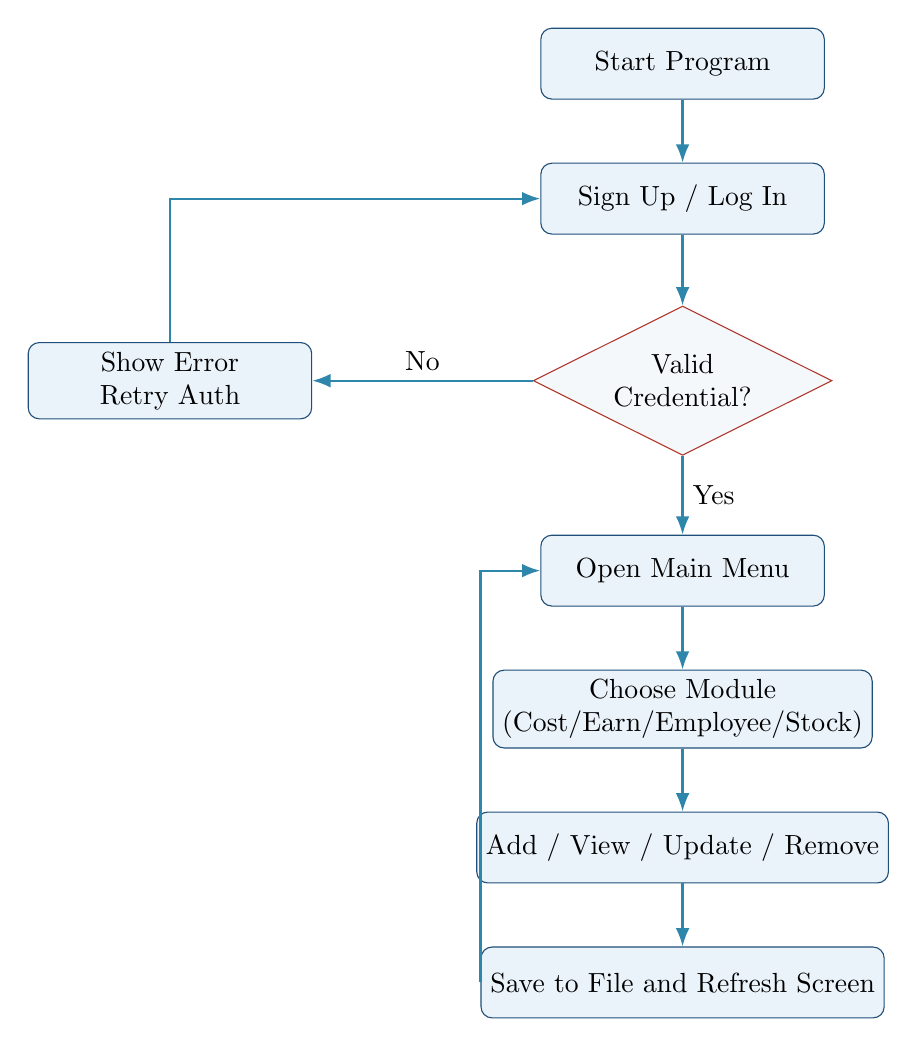
\begin{tikzpicture}[
    node distance=8mm,
    flow/.style={draw=primary,rounded corners,minimum width=36mm,minimum height=9mm,align=center,fill=softblue},
    decision/.style={draw=warn,diamond,aspect=2,align=center,fill=lightbg},
    arr/.style={-Latex,thick,draw=secondary}
]
    \node[flow] (start) {Start Program};
    \node[flow,below=of start] (auth) {Sign Up / Log In};
    \node[decision,below=of auth,yshift=-1mm] (valid) {Valid\\Credential?};
    \node[flow,below=of valid,yshift=-2mm] (menu) {Open Main Menu};
    \node[flow,below=of menu] (module) {Choose Module\\(Cost/Earn/Employee/Stock)};
    \node[flow,below=of module] (op) {Add / View / Update / Remove};
    \node[flow,below=of op] (save) {Save to File and Refresh Screen};
    \node[flow,left=28mm of valid] (retry) {Show Error\\Retry Auth};

    \draw[arr] (start) -- (auth);
    \draw[arr] (auth) -- (valid);
    \draw[arr] (valid) -- node[right]{Yes} (menu);
    \draw[arr] (menu) -- (module);
    \draw[arr] (module) -- (op);
    \draw[arr] (op) -- (save);
    \draw[arr] (save.west) |- (menu.west);
    \draw[arr] (valid.west) -- node[above]{No} (retry.east);
    \draw[arr] (retry.north) |- (auth.west);
\end{tikzpicture}
\end{center}

\section{File and Data Management}
\begin{highlightbox}
\textbf{Design principle: all business data files are user-scoped by filename prefix to isolate records between accounts.}
\end{highlightbox}

\begin{itemize}[leftmargin=1.4em]
    \item Credentials: \texttt{<user\_id>.bin}
    \item Income records: \texttt{<user\_id>\_earn.txt}
    \item Expense records: \texttt{<user\_id>\_costs.txt}
    \item Employee records: \texttt{<user\_id>\_employees.txt}
    \item Stock records: \texttt{<user\_id>stocks.txt}
\end{itemize}

\subsection{Data Format Summary}
\begin{longtable}{|p{3.6cm}|p{3.9cm}|p{6.5cm}|}
\hline
\rowcolor{lightbg}
\textbf{File} & \textbf{Structure} & \textbf{Example} \\
\hline
\texttt{.bin} & password length + raw password bytes & \texttt{[int len][char data...]} \\
\hline
\texttt{\_earn.txt} & item amount date & \texttt{ServiceFee 5000 2026-05-02} \\
\hline
\texttt{\_costs.txt} & item amount date & \texttt{Rent 1500 02-05-2026} \\
\hline
\texttt{\_employees.txt} & id name fields salary status & \texttt{E1 Nafis Ahmed Dhaka 017... 2026-01-02 Manager 45000 0} \\
\hline
\texttt{stocks.txt} & item price quantity & \texttt{Keyboard 850 15} \\
\hline
\end{longtable}

\section{Detailed OOP Analysis (Where Concepts Are Used)}
\subsection{Class Relationship Diagram}
\begin{center}
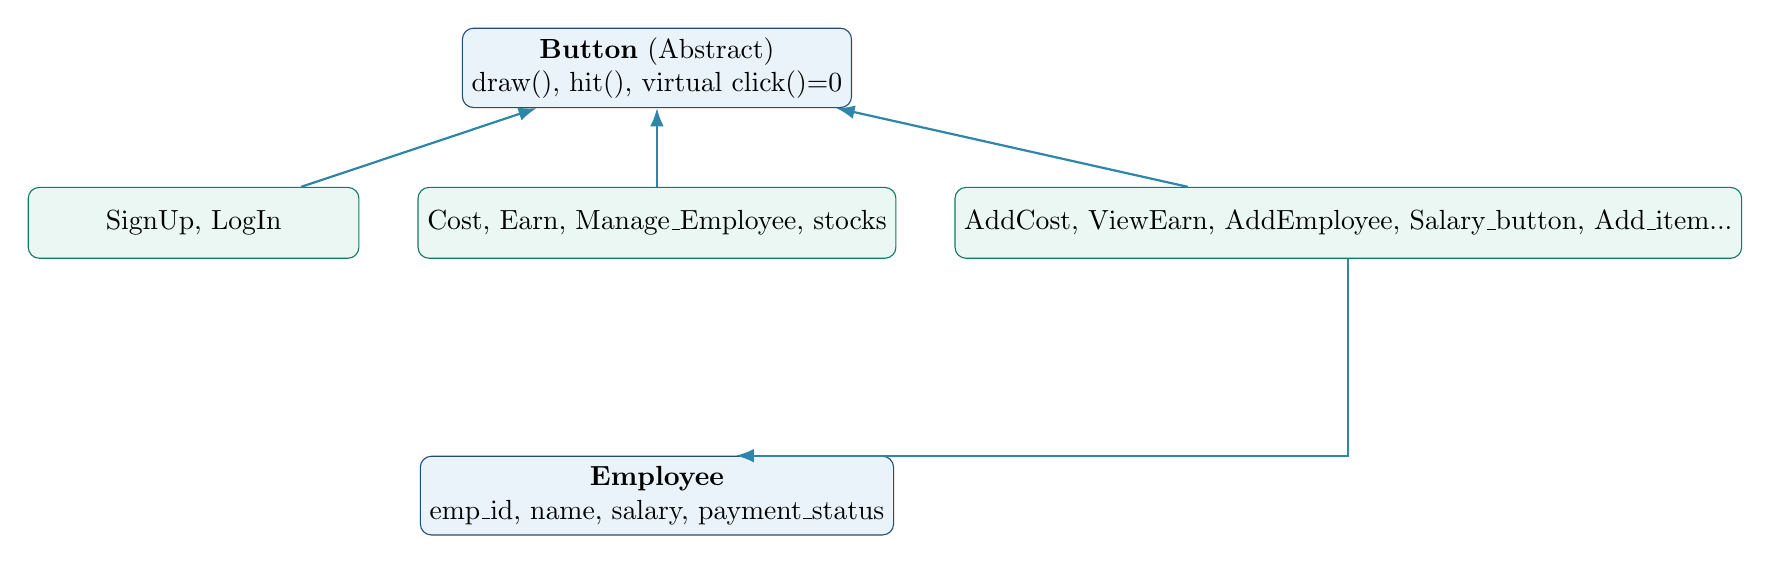
\begin{tikzpicture}[
    node distance=10mm and 13mm,
    cls/.style={draw=primary,rounded corners,minimum width=45mm,minimum height=10mm,align=center,fill=softblue},
    obj/.style={draw=accent,rounded corners,minimum width=42mm,minimum height=9mm,align=center,fill=softgreen},
    arr/.style={-Latex,thick,draw=secondary}
]
    \node[cls] (button) {\textbf{Button} (Abstract)\\draw(), hit(), virtual click()=0};
    \node[obj,below left=of button] (authbtn) {SignUp, LogIn};
    \node[obj,below=of button] (dashboardbtn) {Cost, Earn, Manage\_Employee, stocks};
    \node[obj,below right=of button] (featurebtn) {AddCost, ViewEarn, AddEmployee, Salary\_button, Add\_item...};
    \node[cls,below=25mm of dashboardbtn] (employee) {\textbf{Employee}\\emp\_id, name, salary, payment\_status};

    \draw[arr] (authbtn) -- (button);
    \draw[arr] (dashboardbtn) -- (button);
    \draw[arr] (featurebtn) -- (button);
    \draw[arr] (featurebtn.south) |- ($(employee.north)+(10mm,0)$);
\end{tikzpicture}
\end{center}

\subsection{1) Abstraction}
\begin{itemize}[leftmargin=1.4em]
    \item \texttt{Button} encapsulates generic button behavior (positioning, drawing, click area detection).
    \item Mouse event details are hidden in the reusable \texttt{run()} functions.
    \item Screen modules only define \texttt{click()} behavior and avoid low-level event code repetition.
\end{itemize}

\subsection{2) Inheritance}
\begin{itemize}[leftmargin=1.4em]
    \item Dozens of actionable UI elements are implemented as classes derived from \texttt{Button}.
    \item Examples:
    \begin{itemize}[leftmargin=1.4em]
        \item Authentication: \texttt{SignUp}, \texttt{LogIn}
        \item Dashboard: \texttt{Cost}, \texttt{Earn}, \texttt{Manage\_Employee}, \texttt{stocks}
        \item Feature actions: \texttt{AddEmployee}, \texttt{RemoveEmployee}, \texttt{ViewCost}, \texttt{Update\_item}
    \end{itemize}
\end{itemize}

\subsection{3) Polymorphism}
\begin{itemize}[leftmargin=1.4em]
    \item \texttt{click()} is a pure virtual function in \texttt{Button}, making it an abstract base class.
    \item Different derived classes implement their own runtime click behavior.
    \item In employee management, a \texttt{vector<Button*>} stores mixed button types; dispatch happens via virtual calls.
\end{itemize}

\subsection{4) Encapsulation}
\begin{itemize}[leftmargin=1.4em]
    \item Button coordinate fields are protected and controlled through \texttt{draw()} and \texttt{hit()}.
    \item \texttt{Employee} objects group related employee state for cleaner read/write operations.
\end{itemize}

\subsection{5) Reusability and Modularity}
\begin{itemize}[leftmargin=1.4em]
    \item Shared UI and event logic are reused across all feature screens.
    \item File helpers such as \texttt{get\_employees()} and \texttt{put\_employees()} reduce repeated code.
    \item Header files split declarations from implementation for maintainability.
\end{itemize}

\section{Feature-Level Behavior}
\subsection{Authentication Module}
\begin{itemize}[leftmargin=1.4em]
    \item Sign-up checks for invalid input and duplicate user IDs.
    \item Password is written to a user-specific binary file.
    \item Login validates user existence and matches entered password against stored data.
\end{itemize}

\subsection{Income and Expense Modules}
\begin{itemize}[leftmargin=1.4em]
    \item Add operations append item, amount, date to user-specific text files.
    \item View operations read files and print tabular output.
    \item Income viewer also calculates and displays total earned amount.
\end{itemize}

\subsection{Employee Module}
\begin{itemize}[leftmargin=1.4em]
    \item Supports add, remove, view-details, payment toggle, and reset-all-payment-status.
    \item Uses dynamic action buttons generated per employee record.
    \item Stores payment status as a flag and updates records by rewriting the file.
\end{itemize}

\subsection{Stock Module}
\begin{itemize}[leftmargin=1.4em]
    \item Add operation inserts item name, unit price, quantity.
    \item Update operation loads all records, modifies matching item, then rewrites file.
    \item Remove operation filters out selected item and saves remaining records.
\end{itemize}

\section{Strengths of Current Implementation}
\begin{itemize}[leftmargin=1.4em]
    \item Clear user journey from authentication to business operations.
    \item Good practical use of OOP in a console application context.
    \item Strong modular separation by screen and responsibility.
    \item Persistent, user-scoped data organization.
    \item Visually formatted UI with colorized outputs and structured tables.
\end{itemize}

\section{Limitations and Risks}
\begin{itemize}[leftmargin=1.4em]
    \item Passwords are not hashed or encrypted securely.
    \item Application is tightly coupled to Windows APIs for console interaction.
    \item Validation mostly checks spaces; stronger parsing and range checks are needed.
    \item Dynamic allocations for some runtime buttons are not explicitly released.
    \item Concurrent file access handling and corruption checks are not implemented.
\end{itemize}

\section{Future Enhancements}
\begin{itemize}[leftmargin=1.4em]
    \item Add secure password hashing and account lockout policies.
    \item Refactor dynamic pointers to smart pointers (\texttt{std::unique\_ptr}).
    \item Add summary analytics: monthly profit/loss, top expenses, stock valuation.
    \item Introduce layered architecture (UI, service, repository).
    \item Add export options (CSV/PDF) and search/filter support.
    \item Improve portability by abstracting OS-specific console I/O.
\end{itemize}

\section{Conclusion}
This project successfully demonstrates a complete business-oriented C++ console system with practical OOP usage, persistent file handling, and modular design. The architecture is suitable for academic demonstration and can be evolved into a larger production-ready system by improving security, memory management, portability, and reporting features.

\vspace{1em}
\begin{center}
\color{accent}\rule{0.82\textwidth}{0.5pt}
\end{center}

\end{document}
